% Copyright (c) 2014,2016 Casper Ti. Vector
% Public domain.

\chapter{Data Loader}
Data Loder模块负责图数据的导入,包括点的导入和边的导入。在HybriG架构中,点集数据都存储在Titan中,故点集数据导入直接在Titan上完成。边集数据虽然存储在HBase中,但Titan中的对应边上存储了重边的统计信息,因此需要同时更新Titan和HBase,以保证二者数据的一致。下面详述边的数据导入,以及如何保证Titan和HBase的数据一致性。

\section{边数据的高效导入}
在HybriG架构中,边的插入既要更新Titan,又要更新HBase中的边表。对于给定label的一条边数据,首先要查看Titan中两点间是否已有一条边表示这样的关系存在。若这样的边不存在,则将其创建。然后更新Titan边上的统计信息,再利用其边id将具体边的数据存入HBase中。算法\ref{alg:insert_one_edge}展示了上述逻辑。第1行查询Titan中该label的边,由于至多只有一条,故可用limit(1)加速。第2-4行若这样的边不存在,则在Titan中添加一条边。第5行根据要插入的边数据来更新Titan中边上的统计信息。第6行提交对Titan的所有修改。第7行将边数据写入HBase边表中,行键为e.id拼接上边的主键。
\begin{algorithm}
\caption{插入一条边的伪代码}
\label{alg:insert_one_edge}
\begin{algorithmic}[1] % 每1行显示一个行号
\REQUIRE ~~\\
Titan图接口graph,HBase边表接口hbaseTable,点v1,点v2,edgeLabel,边数据realEdge

\STATE e = v1.query().adjacent(v2).label(edgeLabel).limit(1).edges().next()
\IF{e == null}
\STATE {e = v1.addEdge(v2, edgeLabel)}
\ENDIF
\STATE updateStats(e, realEdge.properties)
\STATE graph.commit()
\STATE hbaseTable.put(e.id + realEdge.primaryKey, realEdge.properties)
\end{algorithmic}
\end{algorithm}

传统的解决方案将所有重边存储在Titan中,边数据的导入逻辑只需要上述代码的第3、5、6行。HybriG架构中每条边的插入多加了一次查询操作(第1行),以及HBase边表的插入操作(第7行),带来了额外的时间开销。而且最耗时的也是这两步操作,分别要从底层存储读取数据以及持久化所有修改到底层存储中。如果有批量重边需要导入,这些开销可以让所有重边来平摊,即在数据导入时,对于两点间同label的重边作为一批来处理,这样就可以共享查询操作的结果,对Titan边上统计信息更新的持久化操作(commit)也只需进行一次。批量导入重边数据的伪代码如算法\ref{alg:insert_batch_edges}所示。
\begin{algorithm}
\caption{重边数据的批量导入}
\label{alg:insert_batch_edges}
\begin{algorithmic}[1] % 每1行显示一个行号
\REQUIRE ~~\\
Titan图接口graph,HBase边表接口hbaseTable,点v1,点v2,edgeLabel,重边数据集allRealEdges

\STATE v1.query().adjacent(v2).label(edgeLabel).limit(1).edges().next()
\IF{e == null}
\STATE e = v1.addEdge(v2, edgeLabel)
\ENDIF
\FOR {realEdge in allRealEdges}
\STATE {updateStats(e, realEdge.properties)}
\ENDFOR
\STATE graph.commit()
\FOR {edge in allRealEdges}
\STATE {hbaseTable.put(e.id + realEdge.primaryKey, realEdge.properties)}
\ENDFOR
\end{algorithmic}
\end{algorithm}

在算法\ref{alg:insert_batch_edges}中,第1到8行是对Titan的更新,将两点间同label的重边作为一批处理,共享了对Titan的操作,从而平摊了额外的开销。另外第9到11行是对HBase边表的多次put操作,可以使用HBase的Bulk Loading 技术来进行加速。

\section{数据一致性}
在Titan的接口设计中,对图(graph)的初次操作将自动打开一个事务,执行graph.commit()时该事务提交,将事务里的修改持久化到底层存储中,Titan的事务保证了自身数据的一致性。HybriG架构由于把边数据的存储分开在Titan和HBase上,需要保证Titan和HBase上数据的一致性。比如Titan上关于重边的统计信息跟HBase边表的一致性,或者HBase边表里各行行键的边id部分跟Titan里的一致性。由于实现强一致性的代价过高,本架构保证的是Titan和HBase数据的最终一致性\supercite{eventually_consistent},即系统保证在经过错误恢复后,数据最终会达到一致的状态。最终一致性足以满足应用场景的需求。
由于只有边集数据是跨Titan和HBase存储的,下面讨论的都是边数据的导入。图\ref{fig:insert_steps}演示了边数据导入的三个步骤,第①步对应前述算法3中的第1~7行,更新Titan数据;第②步对应第8行,提交修改;第③步对应第9~11行,利用边id将边数据插入HBase边表中。对数据的持久化修改是第②③步,数据会出现不一致的原因是②③并不是原子的。如果②成功但是③失败了,即成功持久化了对Titan数据的修改,但对HBase边表的修改却失败了,则两方的数据出现不一致。失败的原因是多种多样的,比如程序内存溢出(Out of Memory)、网络中断、硬件故障等。

\begin{figure}[htbp]
\centering
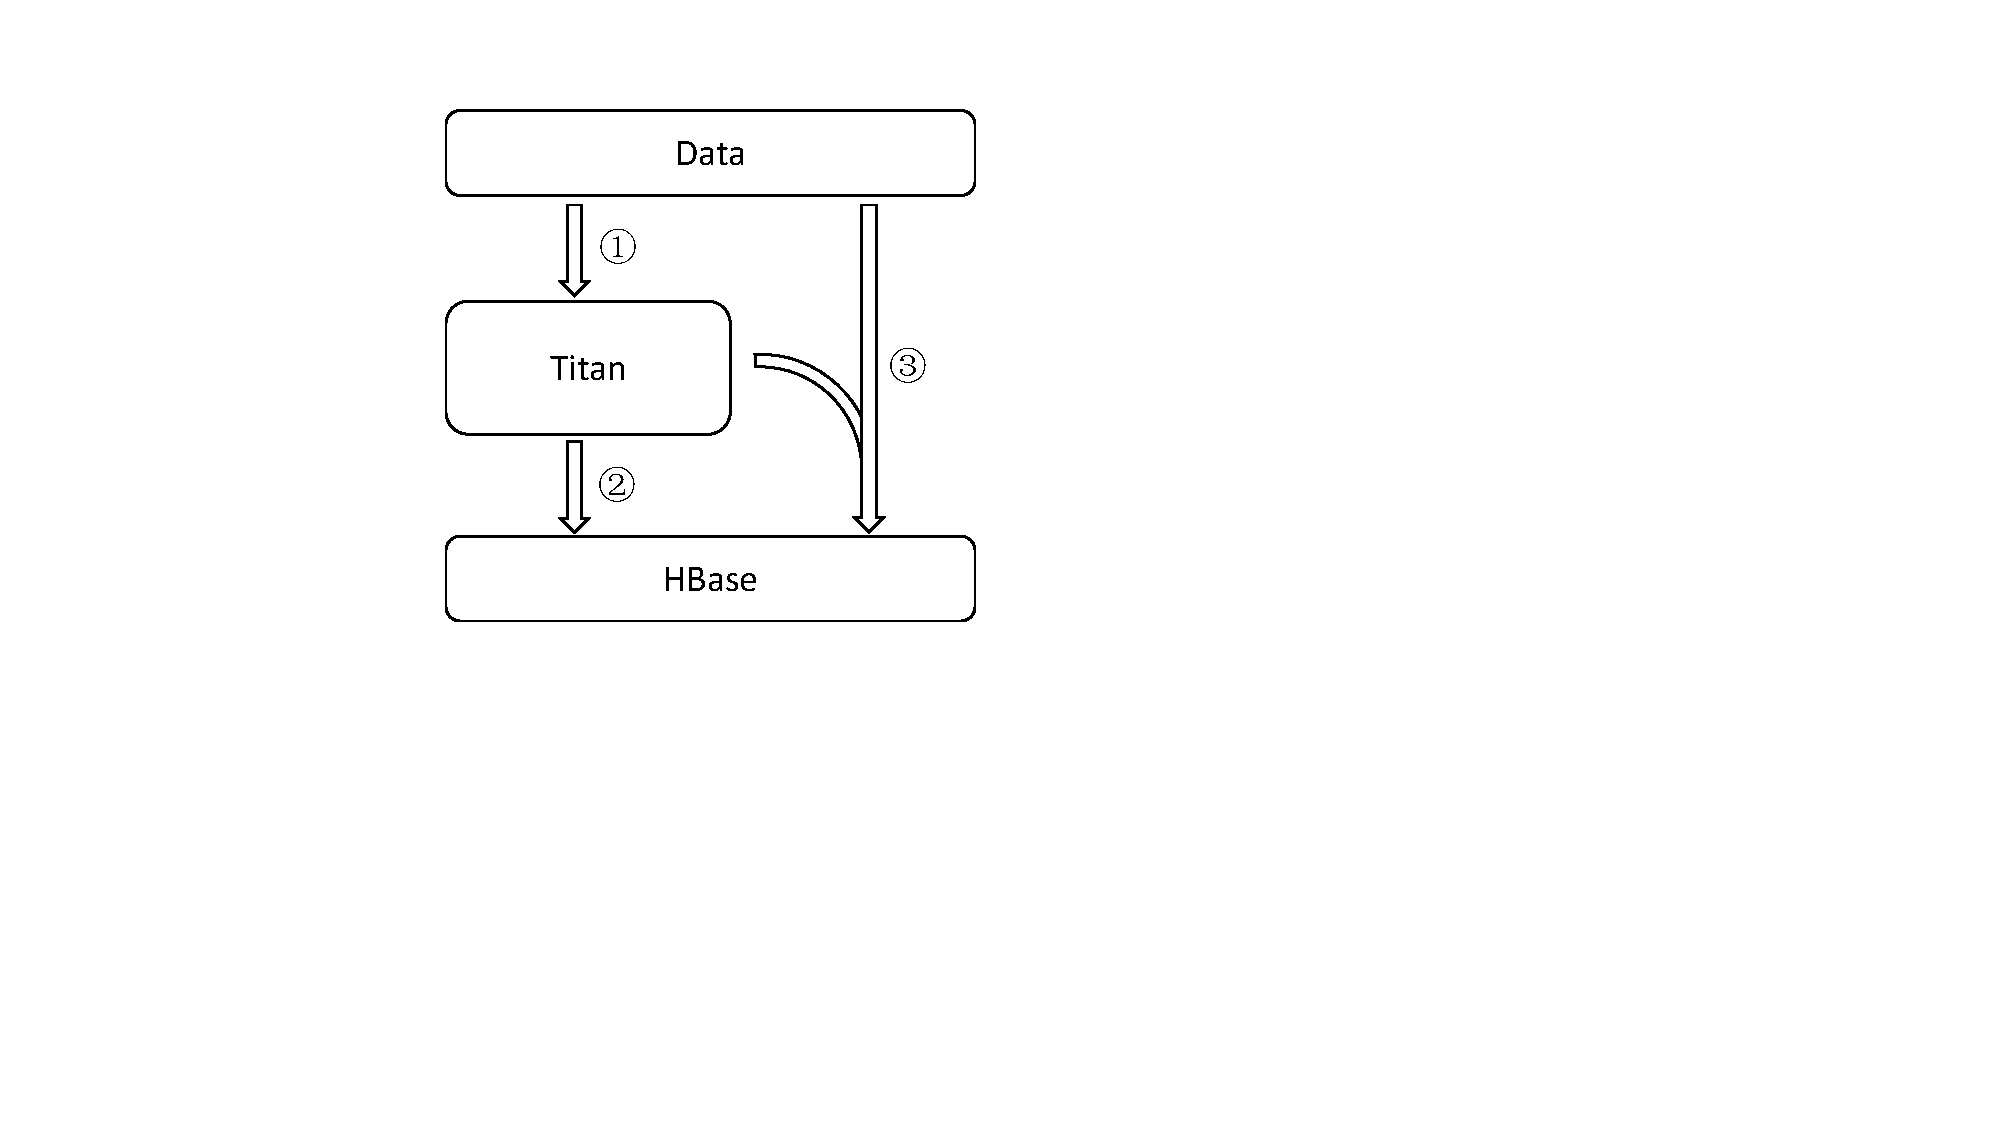
\includegraphics[width=60mm]{fig/insert_steps.pdf}
\caption{边的数据导入分三步:①更新Titan数据;②提交Titan更改即graph.commit();③将数据插入HBase边表中}
\label{fig:insert_steps}
\end{figure}

当数据导入程序在故障之后重启时,这种不一致性需要被修复。该批次的边数据将会被重新导入,为了得知②是否已经成功,我们需要知道Titan中的数据是否已经被修改了。这可以利用Titan的
事务原子性来实现:在②提交之前,往Titan中写入一个成功标志(可以用一个点或属性来表示),然后再提交。根据原子性,该标志被成功写入当且仅当Titan的更新都被持久化。这样当数据导入程序重启时,我们先查看该标志是否存在,便可得知②是否已经成功了。若其已成功,则跳过这一步,直接进行第③步。该过程的伪代码如算法\ref{alg:consistence}所示。

\begin{algorithm}
\caption{保证一致性的边集数据批量导入}
\label{alg:consistence}
\begin{algorithmic}[1] % 每1行显示一个行号
\REQUIRE ~~\\
graph,batchID,HBase边表hbaseTable,点v1,点v2,edgeLabel,allRealEdges,所有边的属性
\STATE e = v1.query().adjacent(v2).label(edgeLabel).limit(1).edges().next()
\IF {hasNotCompleted(graph, batchID)}
	\IF {e == null}
		\STATE {e = v1.addEdge(v2, edgeLabel)}
	\ENDIF
	\FOR {realEdge in allRealEdges}
		\STATE {按需更新边上的统计信息}
	\ENDFOR
	\STATE markCompleted(graph, batchID)
	\STATE graph.commit()
\ENDIF
\FOR {edge in allRealEdges}
	\STATE {hbaseTable.put(e.id + edge.pk, properties)}
\ENDFOR
\end{algorithmic}
\end{algorithm}

算法\ref{alg:consistence}中,第2行的函数hasNotCompleted判断给定的Titan图中是否存在给定批次的成功标志。若不存在则执行第3到10行更新Titan,其中第9行的markCompleted函数在Titan图中插入该批次的成功标志。
值得一提的,我们在HBase中并没有放置成功标志。如果数据导入程序在第③步成功插入HBase数据后出现故障,则重启后还会将边集数据再次插入HBase中。但这是没有问题的,因为HBase边表中的数据不存在统计信息,因此不存在更新操作,所有操作都是新数据的插入操作。我们设置HBase的最大版本数为1,则多次插入同一内容到一个单元格,实际只保存一份,不会增加存储开销。


% vim:ts=4:sw=4
